\chapter{Comparison of Different Approaches}
\section{Comparison of Face Detectors}
The most resource intensive component of the proposed emotion recognition system is the face detection algorithm that constantly scans the input video stream for faces. Multiple approaches were implemented and tested for our use case to determine the optimal algorithm for our system. A qualitative assessment of each algorithm is given in the following section.\\
\begin{minipage}{0.49\textwidth}
\begin{figure}[H]
  \centering
  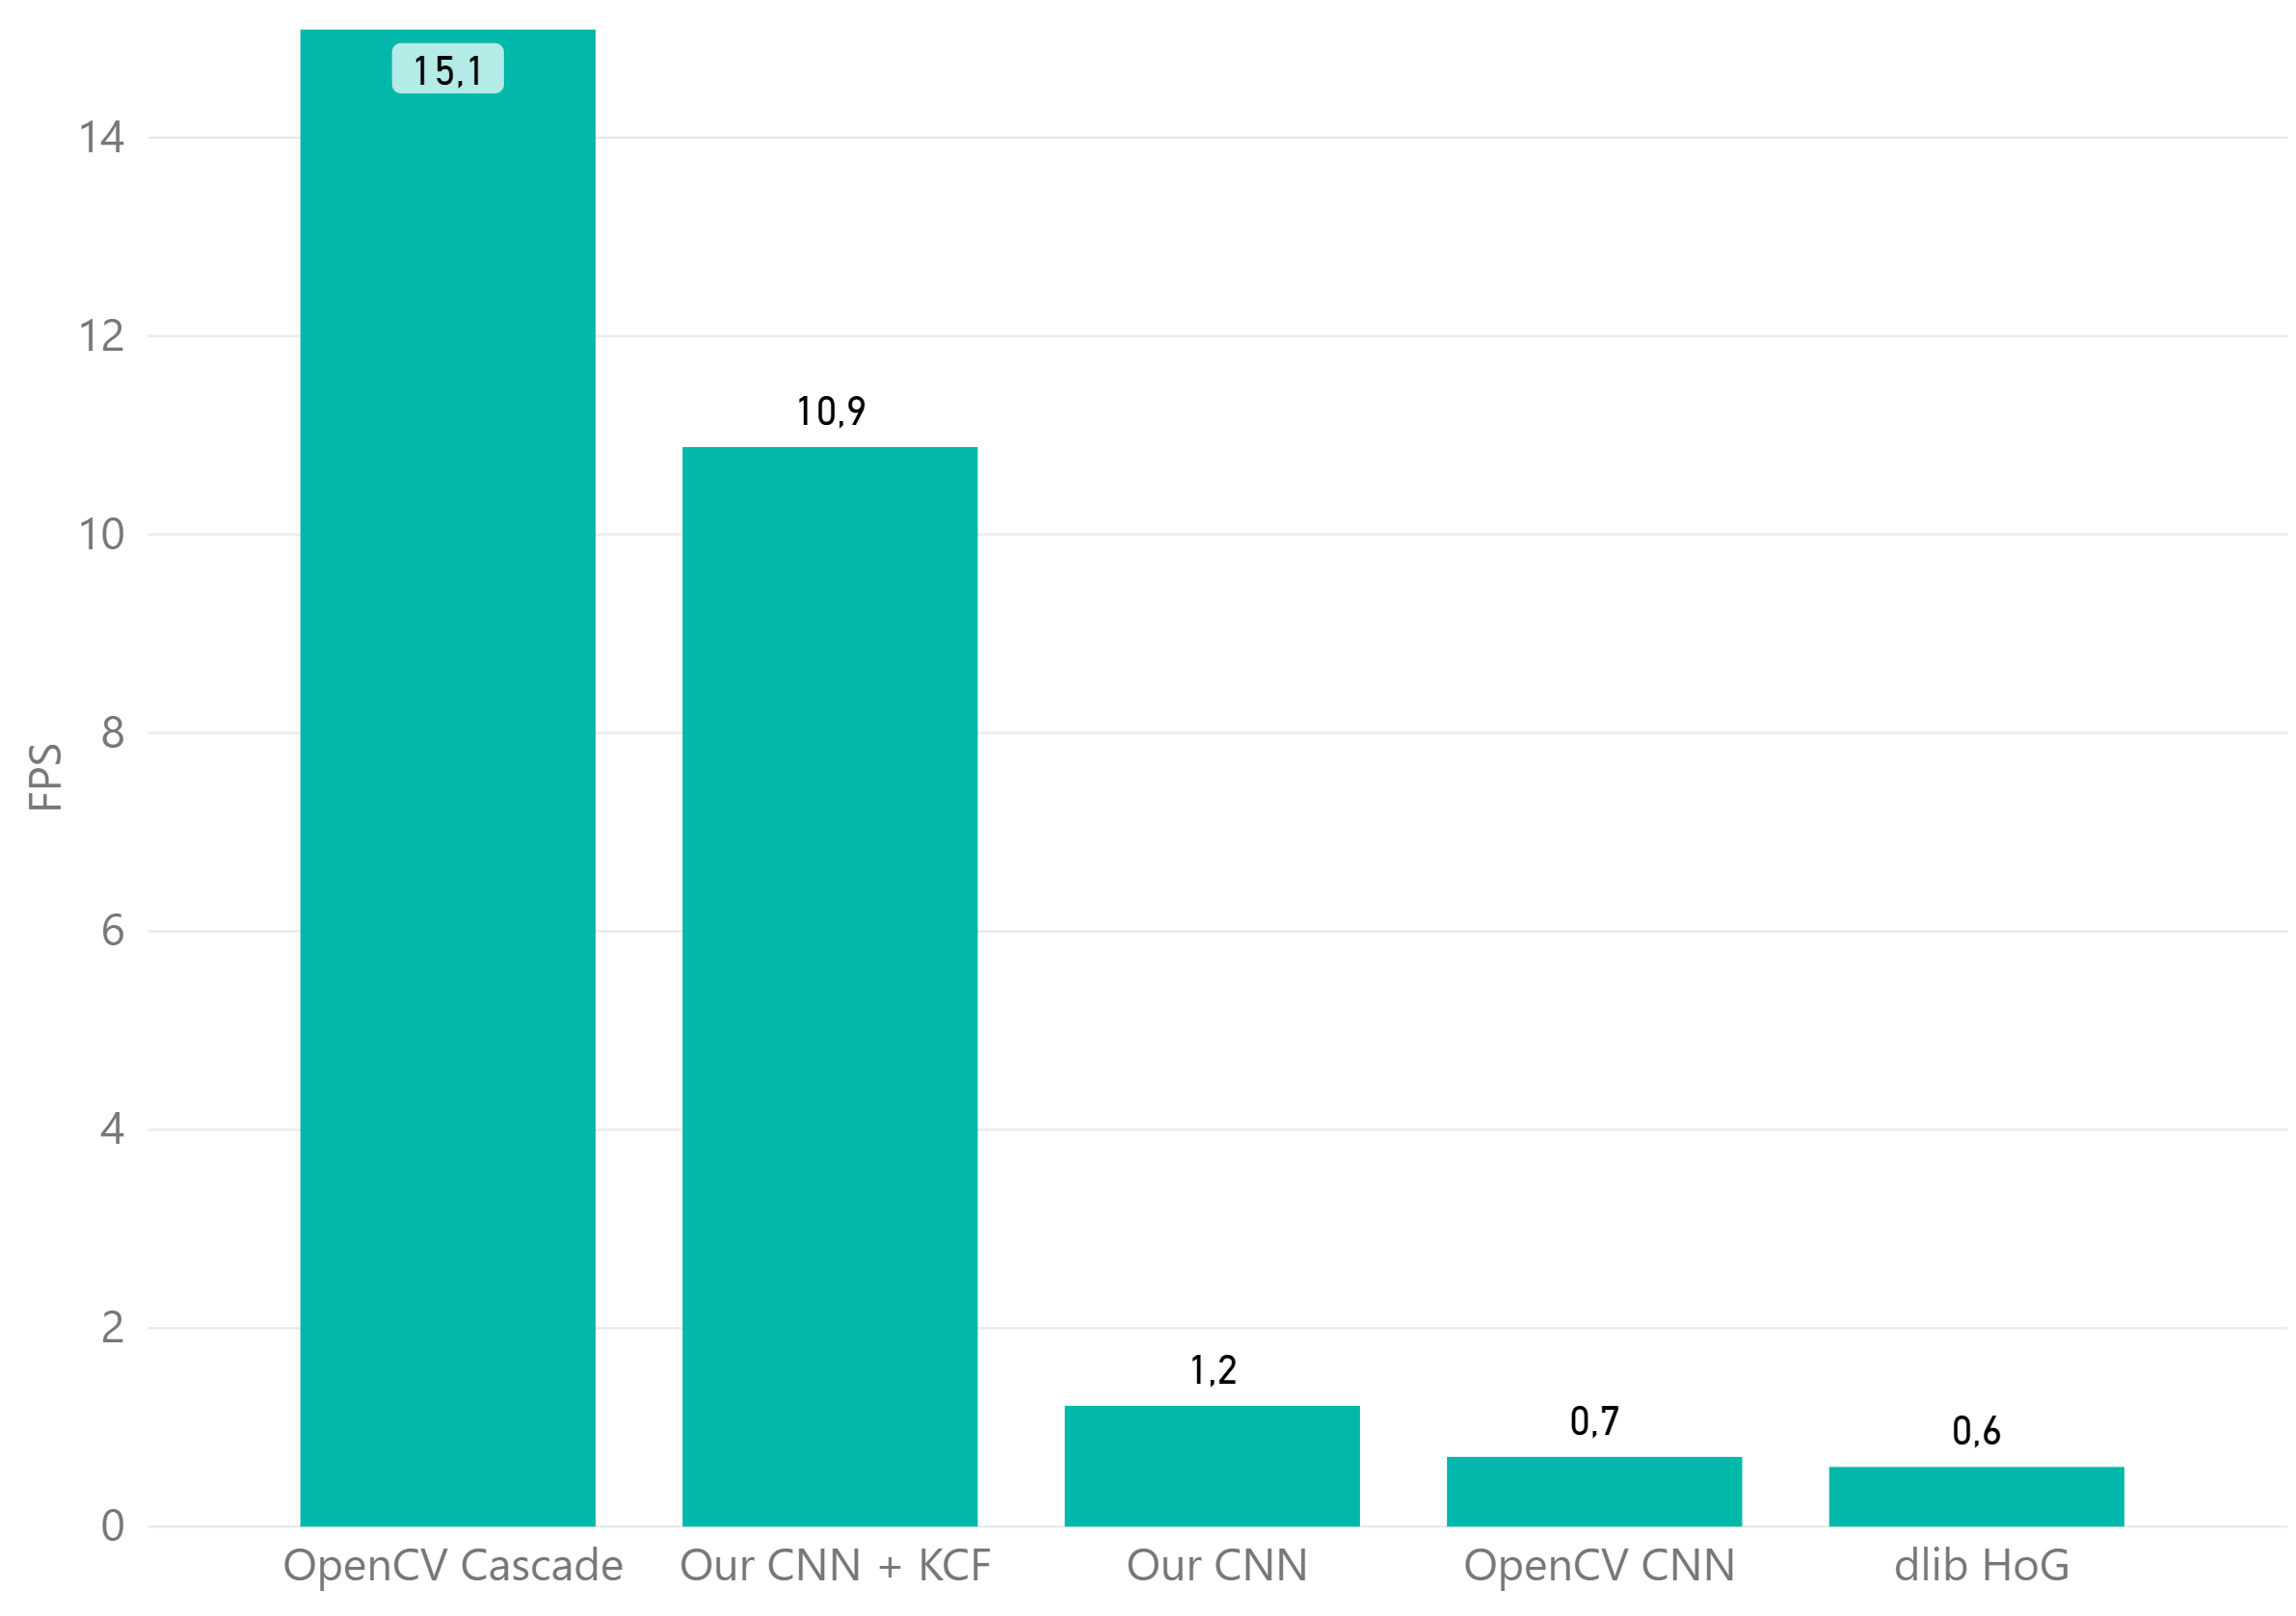
\includegraphics[width=\columnwidth]{media/diagram_FPS.png}
  \caption{Frames per second by approach}
\end{figure}
\end{minipage} \hfill
\begin{minipage}{0.49\textwidth}
\begin{figure}[H]
  \centering
  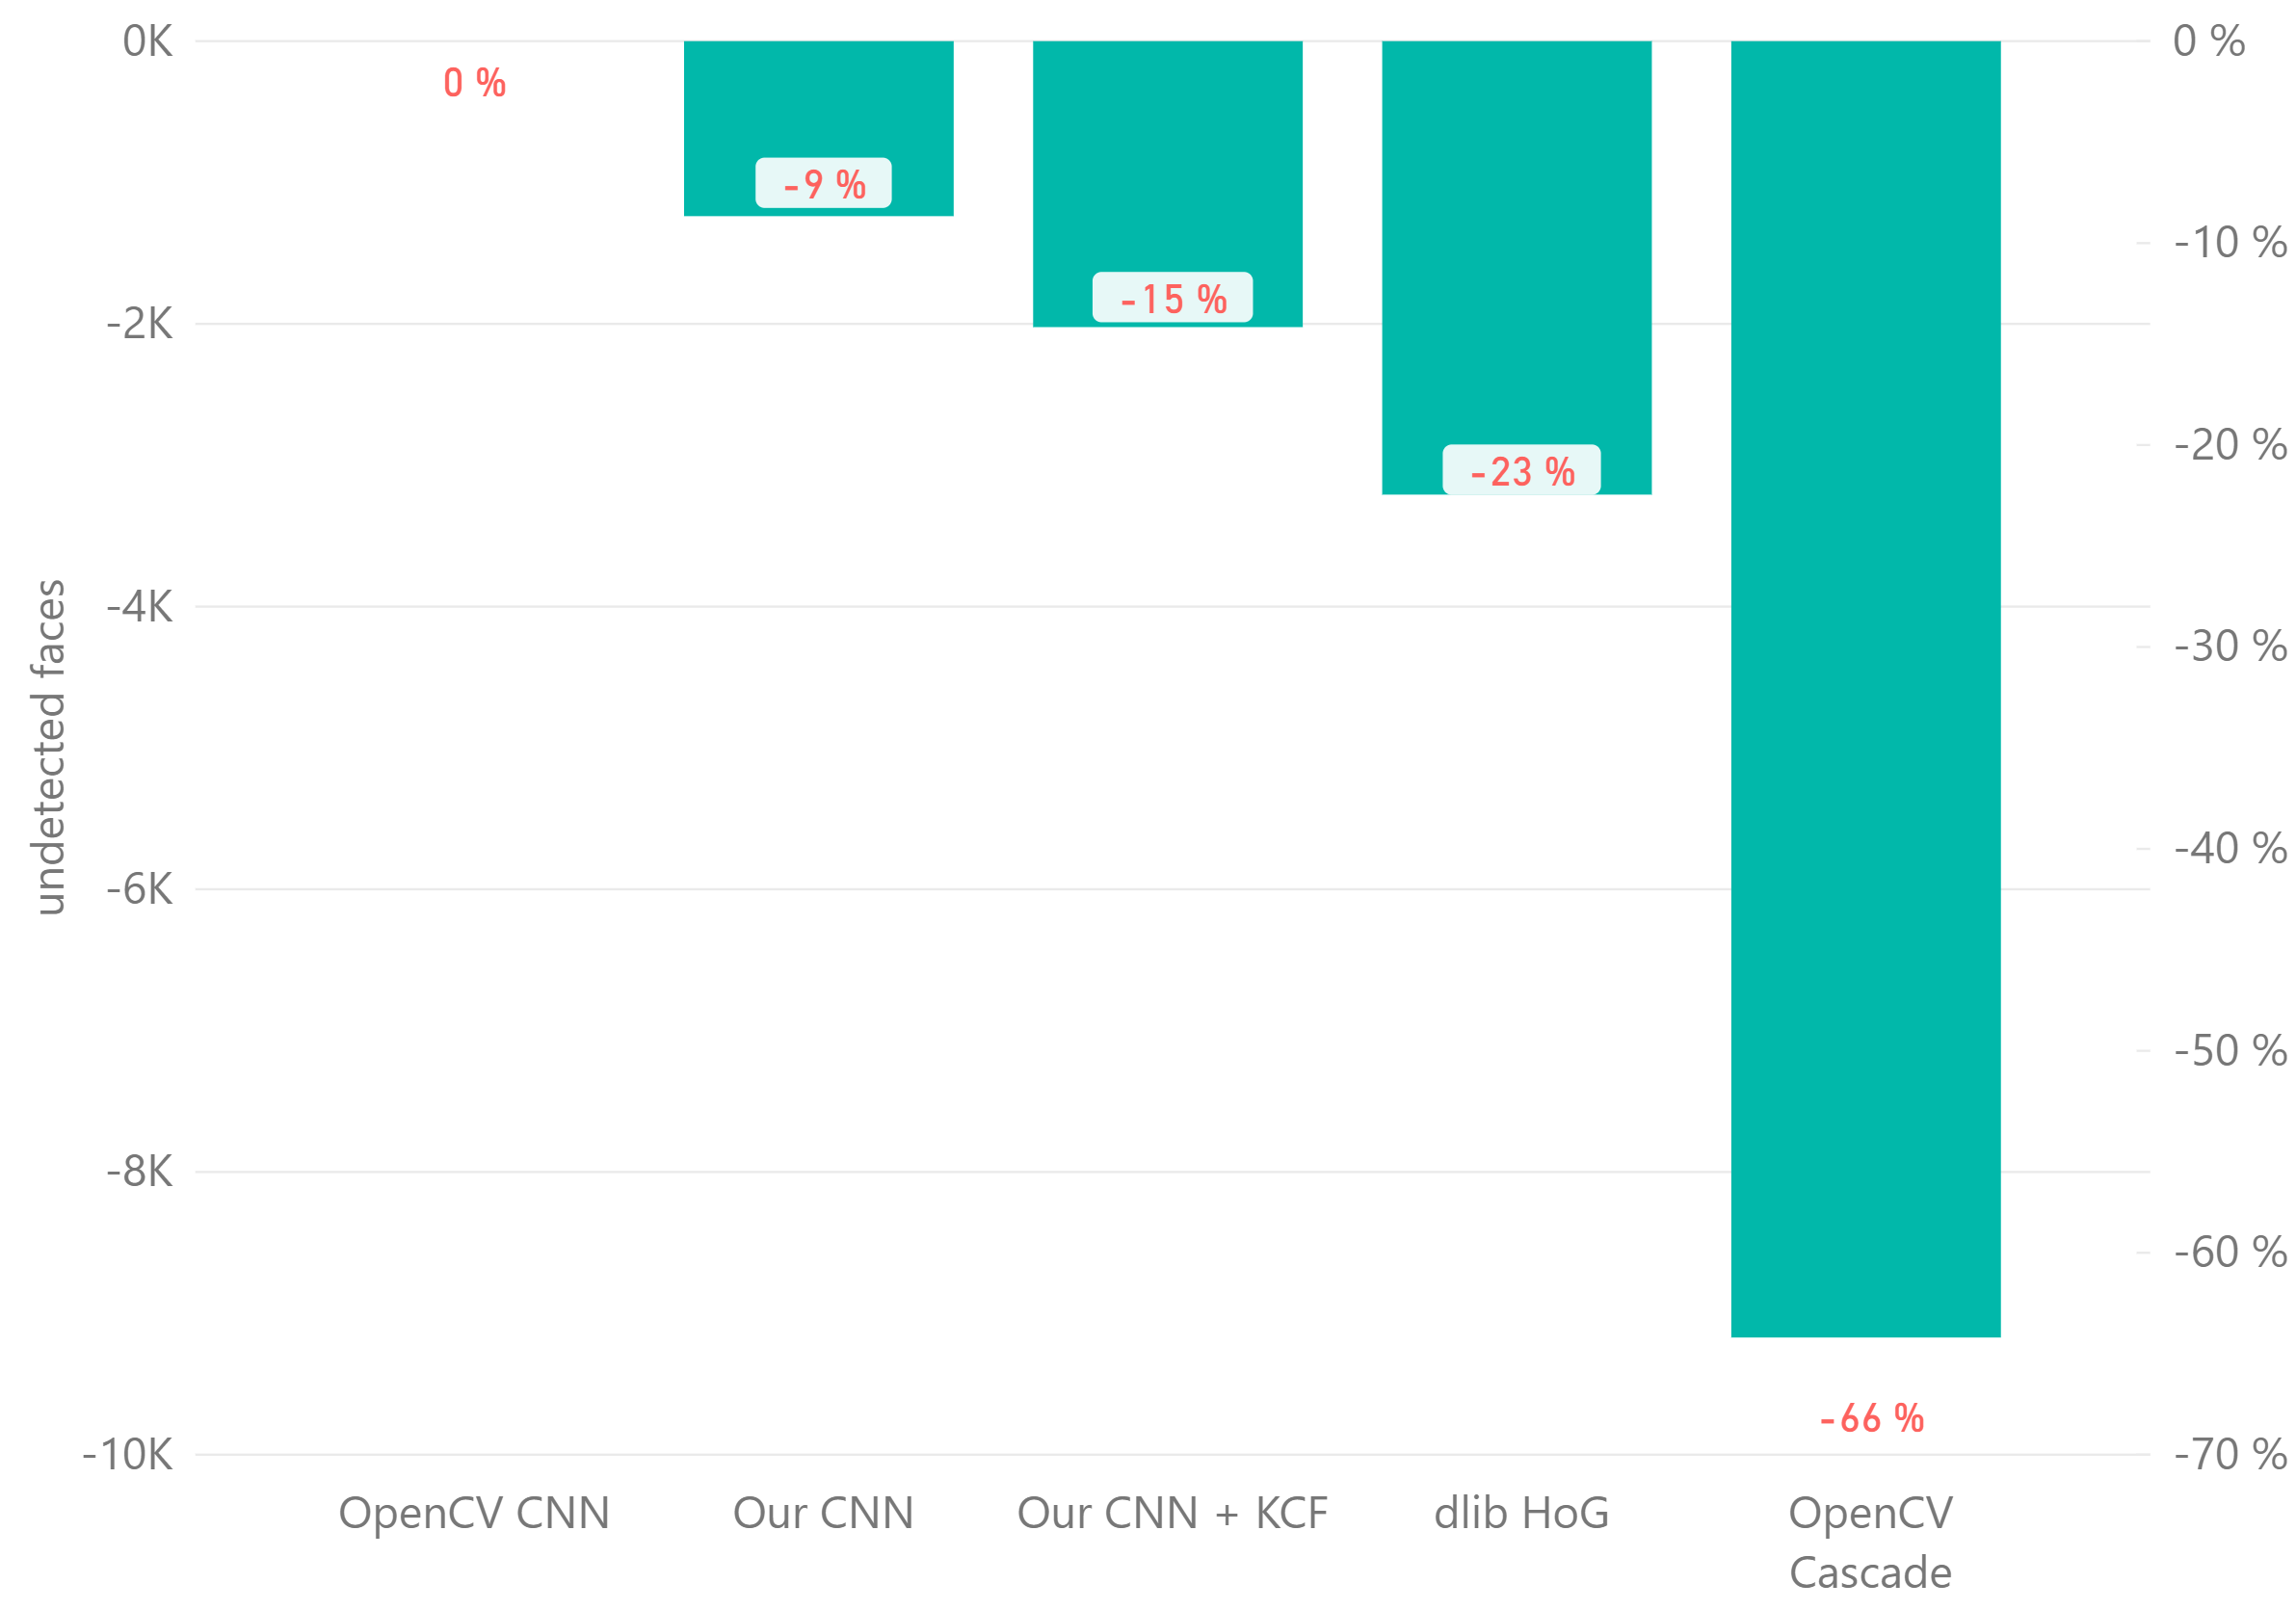
\includegraphics[width=\columnwidth]{media/diagram_accuracy.png}
  \caption{Undetected faces by approach (more details in Evaluation)}
\end{figure}
\end{minipage}
\subsection{Viola Jones Algorithm}
The first implementation tested was the cascading classifier in \gls{opencv} which is based on the Viola Jones Algorithm. Faces are detected in a multistep process that starts by gray scaling the image as color information is not relevant for the algorithm. After that, a Haar Cascade moves over the frame and searches for relevant features. In the last step cascading classifiers eliminate all irrelevant features so that only detected faces are left.\\
The algorithm has a very high performance as it works with integral images and most operations are computationally inexpensive for a CPU. As a result, the algorithm can run at about 15 frames per second on a Raspberry Pi 3.\\%SVM preimplemented%
However, the high performance also comes with significant costs in detection quality as the approach was only able to detect 34\% of the faces in our benchmark video (compared to the pretrained \gls{opencv} neural network) and even slightly tilted faces could not be detected in most cases. Bad lighting or low contrasts as well as occlusion posed an additional challenge.
\subsection{Histogram of Oriented Gradients}
Another implementation that is performant enough to run on an embedded device is the \gls{dlib} \gls{hog} implementation \cite{HoGpaper}. The input stream is converted to a histogram of oriented gradients by calculating contrast deltas in the image. The conversion can utilize CPU optimizations to run as fast as the \gls{opencv} Haar Cascade implementation however it also comes with a significant drawback. The input stream needs to be of much higher resolution for the algorithm to work with small faces. This is a must have for our use case as passengers in the backseats also need to be detected.\\
After fine tuning the parameters to find the optimal resolution for detecting faces up to 1.8m the algorithms performance saw a significant decrease in frames per second and was even outperformed by our \gls{cnn} (0.6 FPS vs. 1.2 FPS).
\subsection{Convolutional Neural Network}
Neural networks can also be used to detect faces and objects in images and video streams. One network architecture that is often used for visual recognition tasks is a \gls{cnn}. \Gls{cnn} use convolutional layers that slide over the image and calculate the dot product of the RGB matrix to extract features and other relevant information. The values are then forwarded through a deep neural network before the output is generated.\\
The model used for our proposed system is based on the SSDLite \gls{mobilenet} architecture. The training process and model details are described in the next chapter. The neural network approach detects almost all faces even under occlusion and with difficult lighting conditions. The only drawback is the relatively high delay of 0.7s (1.2 FPS) on the Raspberry Pi. 

\subsection{Summary of Face Detection Approaches}
\begin{table}[H]
    \resizebox{\textwidth}{!}{%
        \begin{tabular}{|l|l|l|l|l|l|l|}
            \hline
            Approach       & \# Sample Size & Duration & Resolution & FPS  & Detection Quality & Range \\ \hline
            dlib HoG       & 46        & 1.63     & 1000x562   & 0.6  & 77\%     & 1.7 m        \\ \hline
            OpenCV Cascade & 281       & 0.07     & 370x208    & 15.1 & 34\%     & 1.8 m        \\ \hline
            OpenCV CNN     & 94        & 1.42     & 350x196    & 0.7  & 100\%    & 1.9 m        \\ \hline
            Our CNN        & 67        & 0.72     & 350x196    & 1.22 & 91\%     & 1.8 m        \\ \hline
        \end{tabular}%
    }
    \caption[Face Detection Benchmark Results]{Face Detection Benchmark Results}\label{tab:fdm}
\end{table}
Definitions:\\
\begin{itemize}
    \item Sample Size: Number of measurements processed. Note that faster approaches will have a larger sample size for the same test run as they are able to process more frames in the same time.
    \item Duration: Average duration that the algorithm needs to process one frame on the Raspberry PI 3.
    \item Resolution: Resolution of the resized input stream.
    \item FPS: Frames per second on the Raspberry PI 3
    \item Detection Quality: Sum of detected faces in the benchmark video compared to the OpenCV CNN implementation (fixed at 100\% for reference)
    \item Range: Maximum distance between the camera and the person for the face to be detected.\\
\end{itemize}
\section{Comparison of Object Trackers}
Two object trackers were implemented and tested for their performance and accuracy to determine their fit for our application. A qualitative assessment of both is given in the following section.
\subsection{Minimum Output Sum of Squared Error (MOSSE)}
For testing we used the OpenCV implementation of the MOSSE algorithm that is based on the paper "Visual object tracking using adaptive correlation filters". \cite{Mosse} The algorithm runs at about 40 frames per second for tracking one face and can track multiple faces with 25-35 FPS. As there is little occlusion and movement in our use case (mounted camera inside a car) the tracker can reliably track passenger faces with very little failures and interruptions. However, the bounding boxes produced by the algorithm are not precise enough for our use case. The algorithm has problems scaling the bounding boxes with the passengers faces as they change their distance towards the camera. Often this results in a bounding box that only covers a small fraction of the face so that the subsequent facial landmark detection would fail.
\subsection{Kernelized Correlation Filters (KCF)}
In addition to the MOSSE algorithm we also benchmarked the KCF algorithm proposed in the paper "High-Speed Tracking with Kernelized Correlation Filters". \cite{kcf} For testing the \gls{opencv} implementation was used. KCF runs with 15 FPS on the Raspberry PI and provides accurate bounding boxes. However, every additional face reduces the speed by 2-3 FPS so whilst KCF works totally fine for our use case (up to 4 people in a car) it is not recommended for tracking larger groups of people. 
\chapter{Proposed Emotion Recognition System}
\section{System Overview}
\begin{figure}[H]
  \centering
  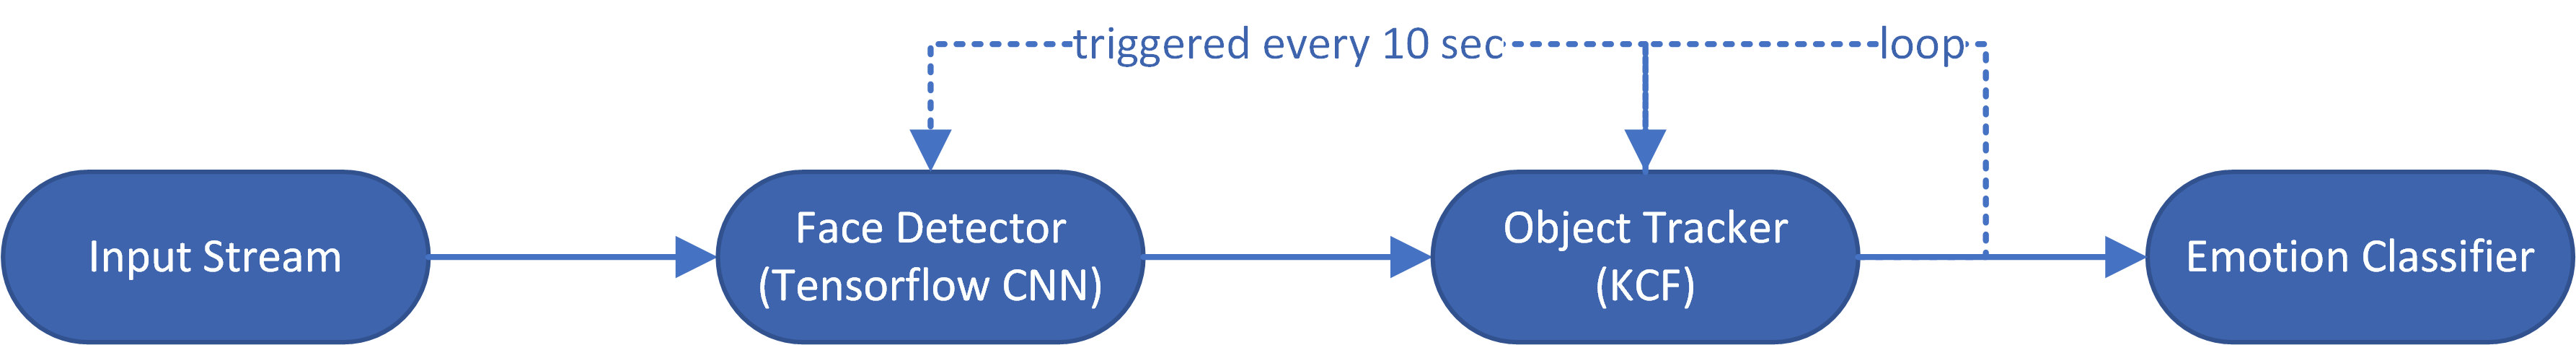
\includegraphics{media/diagram_emotion_detector.png}
  \caption{Processing Pipeline}
  \label{fig:systemmodel}
\end{figure}
The proposed system as shown in Figure \ref{fig:systemmodel} consists of 4 major components. An input stream that is generated by the video capturing device, a \gls{cnn} used as a face detector for detecting the bounding boxes of all faces in the image, a KCF object tracker to subsequently track all detected faces and reduce computational demand and an emotion classifier that interprets the facial landmarks. After optimizing each step, the implementation was able to run on a Raspberry Pi 3 B+ in real-time at 10-15 frames per second, depending on the amount and distance of the detected faces.
\section{Input Stream}
The input stream is generated by the Raspberry Pi camera (V2.1) and has a resolution of 1920x1080 at 30 frames per second. \gls{opencv} is used to open and downscale the stream to 400x224. Additionally frames are buffered to increase performance.
\section{Face Detector}
We decided to use a \gls{cnn} for face detection as the system is required to detect faces in all kinds of different rotations and lightning conditions. This is because our emotion detector is deployed in a car that is expected to have dynamic lighting.\\
The basis for the \gls{cnn} implemented in our final version is the \gls{mobilenet} SSDLite model as found on the \gls{tensorflow} model zoo on GitHub. \cite{modelzoo} \\
The data set used in the training and testing phase is the Wider Face data set. \cite{widerface}\\
As part of the data transformation pipeline small faces and images that contain low quality faces were eliminated from the data set completely so that the final training batch contained about 30.000 faces. The training was performed on 4 Tesla K80 GPUs over 31000 iterations with a final total loss of 2.6.\\
The network input resolution is 300x300 which we found to be the optimal resolution to track faces up to a distance of 1.8m (assumed maximum distance inside a car).
Compared to the \gls{opencv} pretrained model our model offers a 74\% increase in frames per second whilst only detecting 9\% less faces in our benchmark video.
\begin{figure}[H]
  \centering
  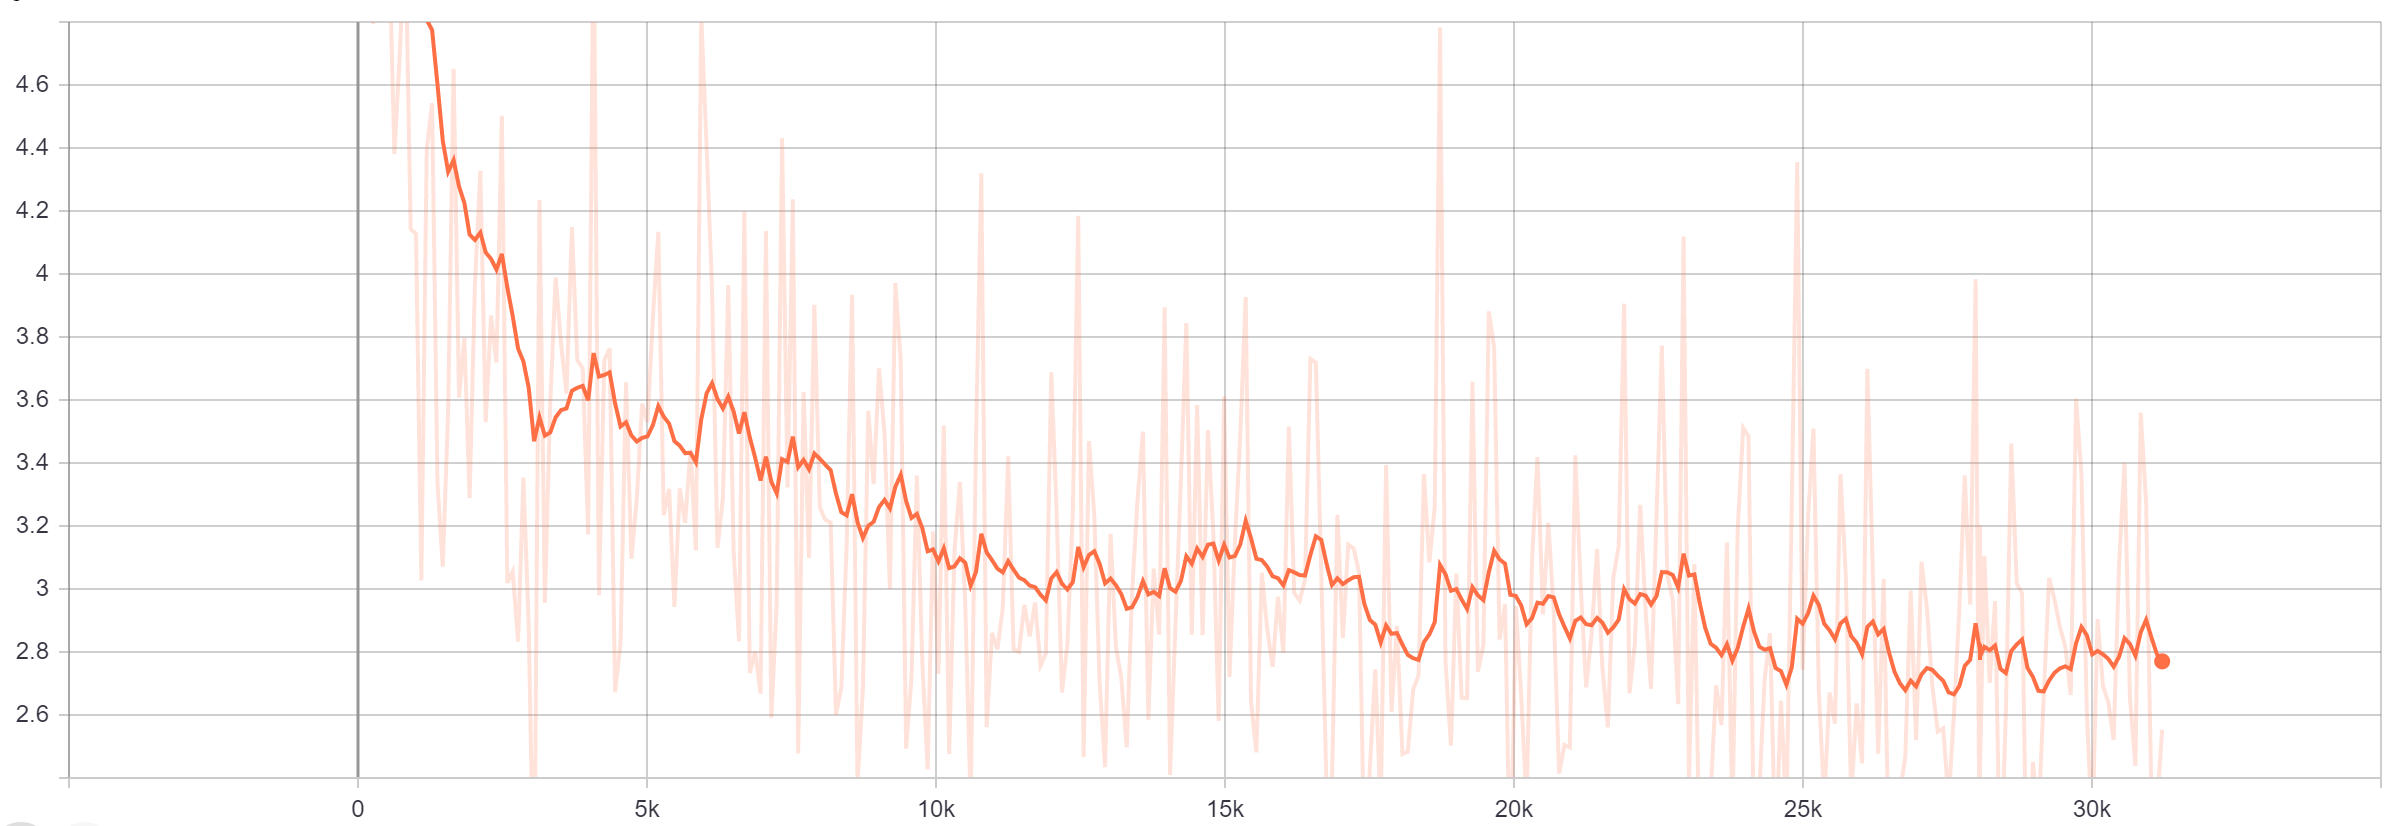
\includegraphics[width=\columnwidth]{media/diagram_Tensorboard.png}
  \caption{Total loss of the trained model (y) over iterations (x)}
\end{figure}
\section{Object Tracker}
We used the KCF object tracker in combination with the Multitracker library provided by OpenCV to track the detected faces. The tracker runs with a slightly higher resolution (400x224) as this significantly improves tracking faces of passengers in the backseat whilst only having a minimal impact on performance compared to the 300x300 resolution used by the \gls{cnn}.\\
The object tracker consumes much less resources compared to the face detection algorithm, however even after extensive fine tuning one problem remains: The sizes of the bounding boxes are not dynamically changing with the face. A way to resolve this problem is to find landmarks in the face and scale the bounding box accordingly (for instance the distance between two eyes would be a scaling factor). A first implementation of this approach showed promising results and the bounding boxes scaled correctly but a few problems still remained. In the end we decided against it as the current facial landmark detector has problems with low-light, low-contrast settings which leads to a significantly lower stability of the system in those cases.
%Bounding box 10% increase
\section{Emotion Classifier}
For emotion classification an existing emotion classifier was used as it only came with the minimal overhead of ~50 ms per face and improving it was out of the scope of this thesis.\\
Before classifying emotions, a facial landmark detector detects 68 facial landmarks with the dlib shape predictor and adds them to a vector. The landmark vector is then passed to a \gls{svm} that was trained in scikit learn on the Extended Cohn-Kanade Dataset \cite{ckplus}. The SVM output provides the the emotion label for each detected face.